\documentclass[a4paper, 10pt]{report}
\usepackage[italian]{babel}
\usepackage[T1]{fontenc}
\usepackage[utf8]{inputenc}
\usepackage{charter}
\usepackage{amsmath}
\usepackage{amsthm}
\usepackage{amsfonts}
\usepackage{graphicx}
\usepackage{wrapfig}
\usepackage{tcolorbox}
\usepackage{fancyhdr}
\usepackage{listings}
\usepackage{longtable}
\usepackage{multicol}
\usepackage{xcolor}

\usepackage{geometry}
\geometry{a4paper, left=2cm,right=2cm,top=2cm,bottom=2cm}

\pagestyle{fancy}
\lhead{}
\chead{}
\rhead{\bfseries 24 ottobre 2019 }
\lhead{\bfseries Segnali e immagini - laboratorio}

\newcounter{main}
\setcounter{main}{1}

\lstnewenvironment{code}[1][firstnumber=\themain,name=main]
  {\lstset{language=matlab,
           basicstyle=\medium\ttfamily,
           numbers=left,
           basicstyle=\small,
           columns=fullflexible,
           #1
          }
}
{\setcounter{main}{\value{lstnumber}}}


\begin{document}

\noindent \textbf{Esempio di Cross correlazione su segnali audio:}

\begin{code}
%% Cross-correlazione su segnali audio: riconoscimento del suono
[Y1,fs1] = audioread('funky.mp3',[1:44100*50]);
[Y2,fs2] = audioread('lost.mp3',[1:44100*50]);
[Y3,fs3] = audioread('Diana.mp3',[1:44100*50]);
[Y4,fs4] = audioread('never.mp3',[1:44100*50]);
[Y5,fs5] = audioread('T69.mp3',[1:44100*50]);

figure; set(gcf,'name','Dataset canzoni','IntegerHandle','off');
subplot(2,3,1); plot(Y1(1:44100*1,1));
subplot(2,3,2); plot(Y2(1:44100*1,1));
subplot(2,3,3); plot(Y3(1:44100*1,1));
subplot(2,3,4); plot(Y4(1:44100*1,1));
subplot(2,3,5); plot(Y5(1:44100*1,1));

%%Array di celle: un metodo piu'veloce per raccogliere sequenze di
%%lunghezza diversa.

gallery{1}=Y1(:,1);
gallery{2}=Y2(:,1);
gallery{3}=Y3(:,1);
gallery{4}=Y4(:,1);
gallery{5}=Y5(:,1);

test=Y2(44100*2:44100*7,:);
\end{code}

\noindent \\Analisi codice:
\begin{longtable}{| p{.25\textwidth} | p{.70\textwidth} |}

\textbf{[Y, FS]=audioread( FILENAME, [START END])} & Legge il file audio FILENAME da START a END (per ogni canale audio). Ritorna i dati campionati in Y e la frequenza di campionamento in FS (in Hz).
\\\\
\textbf{gallery} & Crea un array di "Celle". Una cella è una zona di memoria che può contenere qualsiasi tipo di dato.
\\

\end{longtable}

\noindent Osservazioni:
\begin{itemize}
\item[-] 
\end{itemize}

\noindent Risultato:

\begin{center}
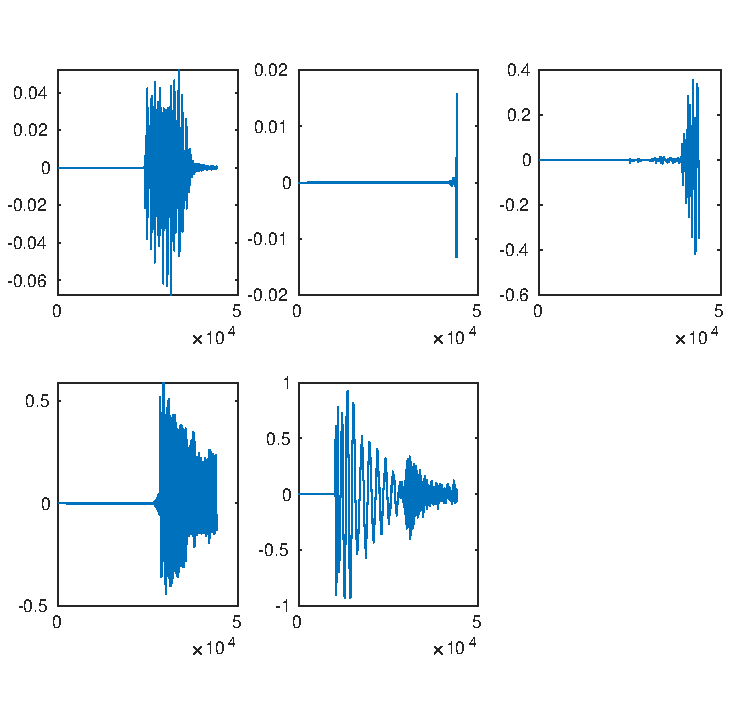
\includegraphics[scale=0.8]{es4.pdf}
\end{center}


\end{document}